% =====================================================================
%  First-year MSc course paper
%  Compile (MiKTeX/TeX Live): pdflatex main -> bibtex main -> pdflatex main x2
%  (Overleaf: builds as-is. Cyrillic Annotation needs T2A, auto-installed.)
% =====================================================================
\documentclass[12pt,a4paper]{article}

\usepackage[utf8]{inputenc}
\usepackage[T1]{fontenc}
\usepackage[a4paper,margin=2.8cm]{geometry}

% --- typography -------------------------------------------------------
\usepackage{amsmath,amssymb}
\usepackage{mathpazo}                 % Palatino text + matching math
\usepackage{microtype}                % professional micro-typography
\linespread{1.10}
\emergencystretch=1.5em

\usepackage{graphicx}
\graphicspath{{figures/}{../results/plots/}}
\usepackage{booktabs}
\usepackage{array}
\usepackage{xcolor}
\usepackage{caption}
\usepackage{tikz}
\usetikzlibrary{arrows.meta,positioning,fit,backgrounds}
\usepackage{enumitem}
\usepackage{placeins}
\usepackage{fancyhdr}
\usepackage[numbers,sort&compress]{natbib}
\usepackage{hyperref}
\hypersetup{citebordercolor={1 0 0}, linkbordercolor={1 0 0}, urlbordercolor={0 0 1}}

% --- accent colour (figures only) ------------------------------------
\definecolor{accent}{HTML}{1F3A5F}

% --- running header ---------------------------------------------------
\setlength{\headheight}{13.6pt}
\pagestyle{fancy}
\fancyhf{}
\renewcommand{\headrulewidth}{0.4pt}
\renewcommand{\sectionmark}[1]{\markboth{\thesection.\ #1}{}}
\fancyhead[L]{\footnotesize\nouppercase{\leftmark}}
\fancyhead[R]{\footnotesize\thepage}

% --- captions & lists -------------------------------------------------
\captionsetup{font=small,labelfont=bf}
\setlist{nosep}

% --- institution details: EDIT THESE FIVE LINES ----------------------
\newcommand{\InstUniversity}{National Research University Higher School of Economics}
\newcommand{\InstFaculty}{International College of Economics and Finance (ICEF)}
\newcommand{\InstDegree}{Bachelor of Science}
\newcommand{\InstSupervisor}{Yaroslav Lyulko}
\newcommand{\InstCity}{Moscow}

% =====================================================================
\begin{document}

% --------------------------- Title page ------------------------------
\begin{titlepage}
\centering
\thispagestyle{empty}
{\large \InstUniversity\par}
{\normalsize \InstFaculty\par}
\vspace{2.6cm}
{\rule{\textwidth}{0.8pt}}\\[0.7cm]
{\LARGE\bfseries Graph-based Analysis of Currency Triangles\\[0.25em]
in FX Markets\par}
\vspace{0.5cm}
{\large Detecting and Exploiting Triangular Arbitrage\par}
\vspace{0.5cm}
{\rule{\textwidth}{0.8pt}}\\[1.6cm]
{\normalsize\itshape A course paper submitted in the first year\\
of the MSc programme\par}
\vfill
{\normalsize
\begin{tabular}{rl}
\bfseries Author: & Nikolay Dvoryanchikov\\[0.35em]
\bfseries Supervisor: & \InstSupervisor\\
\end{tabular}\par}
\vspace{1.2cm}
{\large \InstCity, 2026\par}
\end{titlepage}

% --------------------------- Front matter ----------------------------
\pagestyle{plain}
\pagenumbering{roman}
\setcounter{page}{1}

% ---- Contents (own page) ----
\tableofcontents
\clearpage

% --------------------------- Main matter -----------------------------
\pagestyle{fancy}
\pagenumbering{arabic}

% =====================================================================
\section{Introduction}
\label{sec:intro}

The foreign-exchange market moves trillions of dollars a day, and the banks and treasuries
that operate in it end each day holding currency they never set out to own. Lending,
hedging, and client flow leave every institution with a net position in each currency. That
net position is its open currency position, and it matters: the institution gains or loses
as exchange rates move against that position, and supervisors and internal mandates cap how
large it may grow.

Keeping the open position where it belongs is a standing problem, not a single choice. Rates
change with every quote, so a position that suits an institution one minute suits it less the
next. Pulling it back into line means buying and selling currency, and each trade pays the
gap between bid and ask, so frequent correction drains money even when each trade looks
sound. The currencies move together as well, so a treasurer cannot handle one exposure at a
time. And the treasurer commits to each decision before seeing the next move in rates.

A fixed rule struggles against a problem of this shape. The task asks instead for a way to
decide, again and again and under uncertainty,
how much exposure to carry in each currency while weighing expected return against the cost
of trading and the limits on risk.

Problems with this structure, where an agent acts in sequence, pays for what it does, and
measures success over a horizon instead of a single step, are the domain of reinforcement
learning. An agent of this kind learns a policy from the outcomes of its own decisions and
improves against an objective that reflects what a treasury values.

I propose an agent of this kind for the open currency position. It learns continuous control
with TD3, an actor-critic algorithm in which a critic estimates the value of the current
positions and an actor proposes how to change them. At each step the agent reads the market
together with its own holdings and outputs a shift in exposure across the currencies. Its
reward is the change in portfolio value after the cost of trading, so it learns to seek
return while paying for every adjustment it makes.

Inside this broad task I target one concrete opportunity: triangular arbitrage. When the
rates among three currencies fall out of step, converting from one currency through the other
two and back returns more than it took to begin, a gain that holds until the rates realign.
Spotting the inconsistency is arithmetic. Capturing it is the hard part, because a trader can
run the loop only with currencies already in hand, so the profit depends on what the open
position holds the moment the loop appears. Positioning for it means carrying exposure and
paying spread in advance, with no promise the loop arrives before the rates close. Capturing
arbitrage is therefore part of managing the open position: the same choices about what to
hold, at what cost, under the same uncertainty. I ask whether my agent can learn to hold
the right exposure and seize these loops as they form.

To do that, the agent needs a particular view of the market. A loop spans three currencies at
once, so an agent that reads each currency on its own will miss it; the signal lives in the
connections between currencies. I therefore present the market as a graph, with currencies as
nodes and exchange rates as the edges that join them, and I build the agent's state with a
graph attention network. Attention lets the agent learn which connections to weigh, so it can
recognise a forming loop and judge which currencies are worth holding to fund the loops that
recur. With a graph-attention state, the agent sees the relationships that both the
opportunity and the funding decision depend on.

This paper develops that agent and asks whether, with a graph-attention state, it can manage
the open currency position by detecting and capturing triangular arbitrage.

% =====================================================================
\section{Literature Review and Theoretical Background}
\label{sec:lit}

This section establishes the ideas the project rests on and then places the work in its
literature. The background comes first, in the order the agent uses the ideas: reinforcement
learning, the TD3 algorithm, the foreign-exchange market and triangular arbitrage, and the
graph attention network that draws them together. The literature review follows.

\subsection{Reinforcement learning and Markov decision processes}

Reinforcement learning studies an agent that learns to act by interacting with an
environment~\citep{sutton2018}. At each step $t$ the agent observes a \emph{state} $s_t$, a
description of the current situation; takes an \emph{action} $a_t$; and receives a scalar
\emph{reward} $r_t$ that scores the immediate result. The environment then moves to a new
state and the cycle repeats. The agent's behaviour is its \emph{policy} $\pi$, a rule that
maps a state to an action, and learning means improving that policy from experience alone,
with no teacher supplying the correct action.

The agent does not maximise the next reward but the \emph{return}, the discounted sum of all
rewards from the current step onward,
\begin{equation}
G_t=\sum_{k=0}^{\infty}\gamma^{k}\,r_{t+k},\qquad \max_{\pi}\;\mathbb{E}_{\pi}[\,G_t\,],
\label{eq:return}
\end{equation}
where $r_{t+k}$ is the reward $k$ steps in the future and $\gamma\in[0,1)$ is a \emph{discount
factor} that makes sooner rewards count more than later ones; a value of $\gamma$ near $1$
makes the agent far-sighted. This setup is a \emph{Markov decision process} (MDP), specified
by states, actions, a reward, the probabilities of moving from one state to the next, and
$\gamma$. Its defining assumption, the \emph{Markov property}, is that the next state depends
only on the current state and action, not on the whole history. That assumption matters
directly for me: the state must contain everything relevant to the decision, because a policy
can be no better than the state it is handed. How I turn the market into such a state, the
subject of the graph representation below, is therefore central rather than incidental.

In my project the mapping is concrete. The state is the current market together with the
agent's holdings; the action adjusts the open currency position; the reward is the change in
portfolio value after trading costs; and one step is one tick of market time. Maximising
discounted return then means managing the position well across the whole horizon, not winning
a single trade.

\subsection{Continuous control: actor--critic methods and TD3}
\label{sub:td3}

My actions are continuous: the agent sets real-valued adjustments to its positions rather
than picking from a short list. This rules out methods that score every possible action and
take the best, since there are infinitely many. Actor--critic methods avoid the problem by
splitting the work. An \emph{actor} proposes an action, and a \emph{critic} estimates how good
it is; the critic's estimate tells the actor which way to adjust.

I use Twin Delayed Deep Deterministic Policy Gradient (TD3)~\citep{fujimoto2018td3}. The actor
$\mu_\theta$ is a neural network with parameters $\theta$ that maps a state to one specific
action. The critic $Q_\phi$, with parameters $\phi$, estimates the \emph{value} of taking an
action in a state, meaning the return expected from then on. The actor is trained to produce
actions the critic rates highly, and the critic is trained so its estimates match the rewards
actually received plus the value of the state that follows. TD3 sharpens an earlier algorithm,
DDPG~\citep{lillicrap2016ddpg}, which tends to overestimate values and train unstably. It adds
three corrections, all of which I keep: it trains two critics and trusts the smaller estimate,
which curbs systematic overestimation; it updates the actor less often than the critics, so the
policy follows values only once they settle; and it adds small noise to the action when training
the critic, so the actor cannot latch onto a sharp but spurious peak. Together these make a
stable continuous-control algorithm, which is why I adopt TD3 over the less robust members of
the same family~\citep{silver2014dpg}.

\subsection{The foreign-exchange market and triangular arbitrage}

The agent acts in the spot foreign-exchange market, where one currency is exchanged for another
at a quoted rate. Every pair carries two prices: a \emph{bid}, the rate at which a dealer buys
the base currency from you, and a higher \emph{ask}, the rate at which the dealer sells it to
you. The difference between them, the \emph{spread}, is the cost of transacting, and it is paid
on every leg of every trade.
I write $R(i,j)$ for the executable rate that converts one unit of currency $i$ into currency
$j$ after its spread is paid.

Not every pair is quoted directly. A missing rate can be implied from two others through a
shared currency, giving a \emph{cross-rate}, and the \emph{no-arbitrage} condition requires the
direct and implied rates to agree. \emph{Triangular arbitrage} is the case where that condition
breaks across three currencies. Taking one unit of currency $a$ to $b$, then to $c$, then back
to $a$ leaves the product of the three rates,
\begin{equation}
\phi = R(a,b)\,R(b,c)\,R(c,a),
\label{eq:noarb}
\end{equation}
which I call the \emph{cycle factor}: the multiple of the starting amount held after going
around the loop. Because each conversion already pays its spread, the loop turns a profit
exactly when $\phi>1$, and that profit is $\phi-1$ per unit committed; when $\phi\le 1$ the loop
loses money and is left alone. In real markets such loops are small and disappear within
moments~\citep{fenn2009mirage}. This one number, computed over a three-currency loop, is the
signal the agent must learn to read and act on.

\subsection{The currency graph and graph attention}
\label{sub:graph}

The preceding ideas leave a gap to close. The agent needs a state that captures the market, and
the market's information is relational: a rate links two currencies, consistency ties rates to
each other, and an arbitrage loop spans three currencies at once. A flat list of numbers can
store these quantities but discards how they connect, which is where the signal lives. I need a
representation that keeps the connections, and then a way to turn it into the state vector the
agent reads.

The representation is a \emph{graph}. A graph $G=(V,E)$ is a set of \emph{nodes} $V$ and a set of
\emph{edges} $E$, each edge joining two nodes to record a relationship. When nodes or edges carry
\emph{features}, vectors of numbers describing them, the graph is \emph{attributed}; when an edge
points from one node to another, it is \emph{directed}. A graph is the natural container when the
relationships, rather than the entities on their own, carry the information.

For foreign exchange the mapping is immediate. Each currency is a node, and each executable rate
is a directed edge from one currency to another, since converting $i$ into $j$ differs from the
reverse. The four currencies of this study give four nodes and twelve directed edges, one per
ordered pair (Figure~\ref{fig:graph}). The features hold what the agent needs each tick: a node
carries the currency's current and previous portfolio weight, and an edge carries the rate, its
spread, its recent volatility and momentum, and the arbitrage signal for loops through it. The
triangular loop of the previous subsection is now a three-edge \emph{cycle} in this graph, and
its cycle factor $\phi$ is a property of that cycle. The structure of the market, and the signal
hidden in it, are now explicit in the representation.

\begin{figure}[t]
\centering
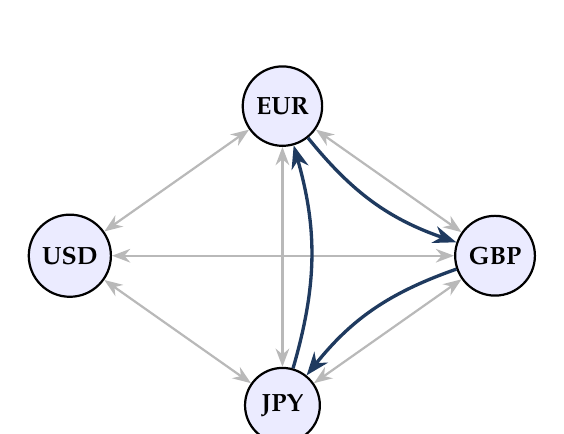
\begin{tikzpicture}[
  >=Stealth,
  ccy/.style={circle,draw,thick,minimum size=0.95cm,font=\small\bfseries,fill=blue!8},
  base/.style={gray!55,<->,thick},
  hl/.style={accent,->,very thick}
]
  \node[ccy] (USD) at (-2.7,0)  {USD};
  \node[ccy] (EUR) at (0,1.9)   {EUR};
  \node[ccy] (GBP) at (2.7,0)   {GBP};
  \node[ccy] (JPY) at (0,-1.9)  {JPY};
  % base pairs: a rate each way (double-headed)
  \draw[base] (USD)--(EUR);
  \draw[base] (USD)--(GBP);
  \draw[base] (USD)--(JPY);
  \draw[base] (EUR)--(GBP);
  \draw[base] (EUR)--(JPY);
  \draw[base] (GBP)--(JPY);
  % one directed 3-cycle, bowed inward
  \draw[hl] (EUR) to[bend right=16] (GBP);
  \draw[hl] (GBP) to[bend right=16] (JPY);
  \draw[hl] (JPY) to[bend right=16] (EUR);
\end{tikzpicture}
\caption{The currency graph as a directed graph for $N=4$. Every pair carries a rate in each
direction, drawn as a double-headed edge, for $N(N-1)=12$ directed edges in all; the accent path
$\text{EUR}\!\to\!\text{GBP}\!\to\!\text{JPY}\!\to\!\text{EUR}$ is one of the eight directed
three-cycles, a triangular-arbitrage loop that pays when its cycle factor $\phi$
of~\eqref{eq:noarb} exceeds one.}
\label{fig:graph}
\end{figure}

A graph is still not the vector a policy can read, and flattening it would discard the structure
just preserved. A \emph{graph neural network} turns the graph into vectors while respecting its
connections, through \emph{message passing}~\citep{gilmer2017mpnn,battaglia2018relational}. Each
node starts from its feature vector and refines it over rounds; in each round a node gathers its
neighbours' current vectors, combines them into one message, and updates its own vector from that
message. With $h_i^{(l)}$ the vector of node $i$ after round $l$,
\begin{equation}
h_i^{(l+1)}=\operatorname{update}\!\Big(h_i^{(l)},\ \operatorname{aggregate}\big\{\,h_j^{(l)}:j\text{ adjacent to }i\,\big\}\Big),
\end{equation}
where \emph{aggregate} fuses the neighbours and \emph{update} folds the result back into the
node. Stacking $L$ such rounds carries information up to $L$ steps across the graph, so each
currency's vector comes to reflect the currencies it connects to, not itself alone.

How a node weights its neighbours decides what that message carries, and for me it is the whole
point. The simplest networks weight every neighbour equally, or by a fixed rule based on how many
connections each node has~\citep{kipf2017gcn}. My signal is the opposite of uniform: at any tick
the three edges of a mispriced loop matter and the rest are noise, so equal weighting averages
the few informative edges in with many uninformative ones and dilutes exactly what the agent
should see. A \emph{graph attention network} (GAT) removes this limitation by learning the
weights and letting them depend on the content of the
nodes~\citep{velickovic2018gat,brody2022gatv2}. For each neighbour $j$ of node $i$ it computes an
\emph{attention weight} $\alpha_{ij}\in[0,1]$ saying how much $j$ should count for $i$, then
updates $i$ as a weighted sum,
\begin{equation}
\alpha_{ij}=\operatorname{softmax}_j\big(\operatorname{score}(h_i,h_j)\big),\qquad
h_i'=\sigma\Big(\textstyle\sum_{j}\alpha_{ij}\,W h_j\Big),
\label{eq:gat}
\end{equation}
where \emph{score} is a small learnable function comparing two nodes, $\operatorname{softmax}_j$
normalises the weights over $i$'s neighbours so they sum to one, $W$ is a learned matrix that
transforms each neighbour's vector, and $\sigma$ is a non-linearity. Several independent
weightings, called \emph{attention heads}, run in parallel, so a node can attend to more than one
relationship at once.

Because the deciding quantities in my market sit on the edges, I feed the edge features into
\emph{score}: the weight a currency places on a neighbour then depends on the rate, spread, and
arbitrage signal that connect them, and the attention can settle on the edges of a loop that is
currently live. The network returns one refined vector per currency, and these are concatenated
into the single state vector that the TD3 actor and critic consume. This is the state the MDP
demanded: the graph holds the market's structure, attention keeps the part that matters, and the
result is what the agent acts on.

\subsection{Literature review}
\label{sub:litreview}

I now look at how others have approached the parts of this problem, what they found, and
where my plan sits among them. Three lines of work bear on it directly: reinforcement
learning for trading and portfolio control, graph models of financial markets, and the study
of arbitrage.

Reinforcement learning reached trading through direct, or recurrent, reinforcement learning.
Moody and Saffell trained a policy online to maximise the differential Sharpe ratio with
transaction costs written into the objective, and showed two things that still hold:
optimising the policy directly works better than learning a value function and then acting on
it, and realistic costs change the shape of the policy rather than trimming its
edges~\citep{moody2001}. Deng et al.\ kept that direct-policy idea but learned the input
features with a deep network instead of choosing them by hand, and improved trading on real
futures and stocks~\citep{deng2017}. Jiang et al.\ turned to allocation across many assets:
their agent scores each asset with an identical sub-network and carries a memory of the
previous weights so that rebalancing has a price, and in a cryptocurrency backtest it
multiplied its capital several times over fifty days even under a $0.25\%$
commission~\citep{jiang2017portfolio}. Liang et al.\ set the continuous-control algorithms
side by side on Chinese equities, reported that a plain policy gradient trained more reliably
than DDPG or PPO, and raised return and Sharpe with adversarial price
perturbations~\citep{liang2018adversarial}; the fragility they saw in DDPG is the weakness the
TD3 stabilisers of Section~\ref{sub:td3} were built to fix. Tsai and Wang carried the approach
to currencies, turning each price window into a Gramian Angular Field image, driving a
Sure-Fire statistical-arbitrage rule, and comparing DQN against PPO on three FX
pairs~\citep{tsai2019fxrl}. These systems share one trait that bears on me: each reads a flat
or per-asset state, so the relations among currencies stay implicit and arbitrage never
reaches the action. I keep their durable lessons, a cost-aware risk-adjusted reward and a
continuous policy, and change exactly that state.

The missing relations are what graph models add. Feng et al.\ ranked stocks with a temporal
model joined to a graph convolution over relations drawn from sector membership and corporate
links, and found that the relations improved both the ranking and its simulated return over
models that ignore them~\citep{feng2019temporal}. Shi et al.\ moved the graph inside the
reinforcement-learning loop: their GPM agent extracts inter-asset relations with a relational
graph convolution, combines them with multi-scale temporal features, and outperforms
non-relational portfolio agents~\citep{shi2022gpm}, and graph-based reinforcement learning for
portfolios has stayed active since. The pattern is consistent, a relational state helps a
learning trader, but two gaps remain for me. These studies live in equities, and their edges
stand for similarity or economic kinship, whereas an FX edge is an executable conversion rate,
and a closed loop of such rates is exactly where arbitrage appears, the structure I set up in
Section~\ref{sub:graph}.

Arbitrage itself has been studied mostly as a detection problem. The statistical-arbitrage
tradition descends from Engle and Granger, who showed how to fix a stationary combination of
prices and trade its deviations, a structure the modeller specifies rather than
learns~\citep{engle1987cointegration}. Triangular arbitrage is the deterministic,
cross-sectional version, and the evidence on it is cautionary: measuring executable spot-FX
quotes, Fenn et al.\ found gaps below one basis point that close in under a second and have
grown scarcer as trading electronified, so winning enough of them to profit is
unrealistic~\citep{fenn2009mirage}. Graph learning has reached this corner too: Hong and
Klabjan model currencies as nodes and rates as edges, forecast the rates with a
spatiotemporal graph network, and choose statistical-arbitrage trades by constrained
optimisation that accounts for execution delay, reporting a large gain in information ratio
over their benchmarks~\citep{hong2025graphfx}. This body of work detects the inconsistency, or
predicts the prices around it; it does not learn a policy that decides how much to commit and
which currencies to hold in order to capture it.

My plan sits where these lines meet, and it differs from each in a definite way. Where
reinforcement-learning traders read a flat state, I read the currency graph of
Section~\ref{sub:graph}; where graph models in finance encode similarity among equities, my
edges are executable FX rates whose cycles carry the arbitrage; and where the arbitrage
literature detects or forecasts, my agent acts, allocating exposure and capturing the loops
the graph reveals through the TD3 controller of Section~\ref{sub:td3}. How I test this
plan, and against what reference, belongs to the experimental sections that follow, and I
settle it there rather than prejudge it here.

% =====================================================================
\section{Model and Methodology}
\label{sec:model}

\begin{figure}[t]
\centering
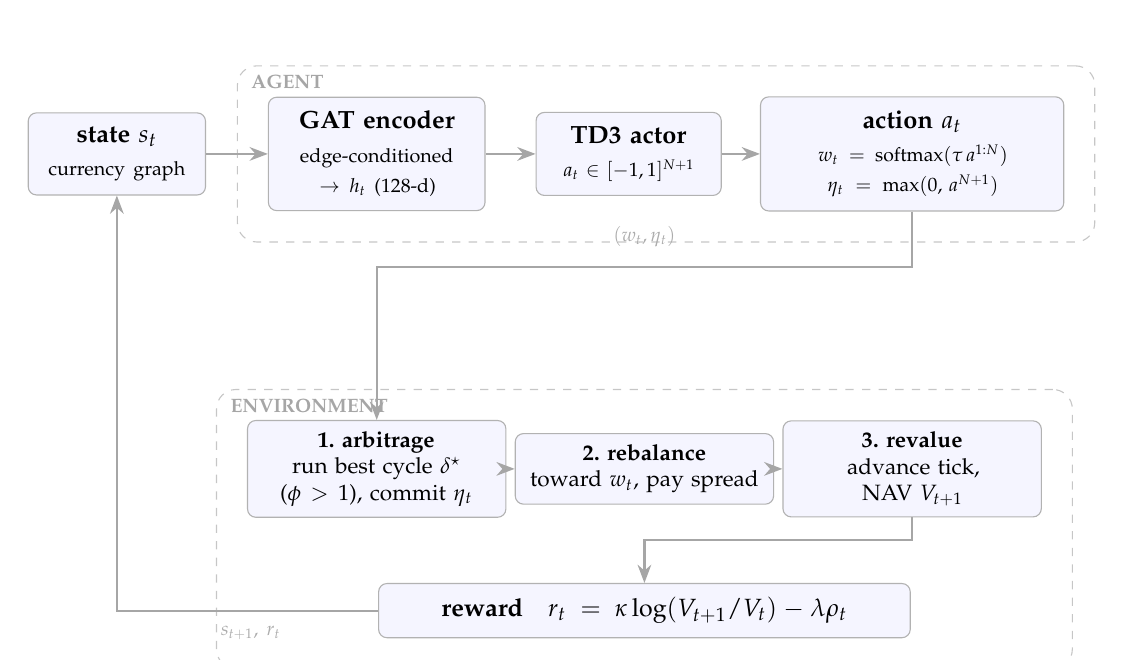
\begin{tikzpicture}[
  >=Stealth, font=\small,
  box/.style={draw=gray!60, rounded corners=3pt, align=center, inner sep=5pt, fill=blue!4},
  estep/.style={draw=gray!60, rounded corners=3pt, align=center, inner sep=4pt, fill=blue!4,
               text width=3.0cm, font=\footnotesize},
  grp/.style={draw=gray!45, dashed, rounded corners=7pt, inner sep=11pt},
  flow/.style={->, thick, gray!70},
  elab/.style={font=\scriptsize\itshape, text=gray!65}
]
  \node[box, text width=1.9cm] (state) at (0,2.3)
    {\textbf{state} $s_t$\\[1pt]{\scriptsize currency graph}};
  \node[box, text width=2.4cm] (gat) at (3.3,2.3)
    {\textbf{GAT encoder}\\[1pt]{\scriptsize edge-conditioned}\\{\scriptsize $\to h_t$ ($128$-d)}};
  \node[box, text width=2.0cm] (actor) at (6.5,2.3)
    {\textbf{TD3 actor}\\[1pt]{\scriptsize $a_t\in[-1,1]^{N+1}$}};
  \node[box, text width=3.5cm] (act) at (10.1,2.3)
    {\textbf{action} $a_t$\\[1pt]{\scriptsize $w_t=\operatorname{softmax}(\tau\,a^{1:N})$}\\{\scriptsize $\eta_t=\max(0,\,a^{N+1})$}};
  \node[estep] (e1) at (3.3,-1.7)
    {\textbf{1.\ arbitrage}\\run best cycle $\delta^\star$ ($\phi>1$), commit $\eta_t$};
  \node[estep] (e2) at (6.7,-1.7)
    {\textbf{2.\ rebalance}\\toward $w_t$, pay spread};
  \node[estep] (e3) at (10.1,-1.7)
    {\textbf{3.\ revalue}\\advance tick, NAV $V_{t+1}$};
  \node[box, text width=6.4cm] (rew) at (6.7,-3.5)
    {\textbf{reward}\quad $r_t=\kappa\log(V_{t+1}/V_t)-\lambda\rho_t$};
  \draw[flow] (state)--(gat);
  \draw[flow] (gat)--(actor);
  \draw[flow] (actor)--(act);
  \draw[flow] (act.south) -- ++(0,-0.7) -| (e1.north);
  \node[elab] at (6.7,1.25) {$(w_t,\eta_t)$};
  \draw[flow] (e1)--(e2);
  \draw[flow] (e2)--(e3);
  \draw[flow] (e3) -- ++(0,-0.9) -| (rew.north);
  \draw[flow] (rew.west) -| (state.south);
  \node[elab] at (1.7,-3.78) {$s_{t+1},\ r_t$};
  \begin{scope}[on background layer]
    \node[grp, fit=(gat)(actor)(act)] (agentbox) {};
    \node[grp, fit=(e1)(e2)(e3)(rew)] (envbox) {};
  \end{scope}
  \node[font=\scriptsize\bfseries, text=gray!70, anchor=north west] at (agentbox.north west) {~AGENT};
  \node[font=\scriptsize\bfseries, text=gray!70, anchor=north west] at (envbox.north west) {~ENVIRONMENT};
\end{tikzpicture}
\caption{The system as one decision loop. The currency-graph state $s_t$ is encoded by the graph
attention network into a vector $h_t$, and the TD3 actor maps it to an action that splits into a
target allocation $w_t$ and an arbitrage intensity $\eta_t$. The environment runs the best
profitable cycle $\delta^\star$ at intensity $\eta_t$, rebalances toward $w_t$ while paying the
spread, advances one tick and revalues to $V_{t+1}$, and returns the next state $s_{t+1}$ and the
reward $r_t$.}
\label{fig:system}
\end{figure}

\subsection{The Markov decision process}

Single-account FX portfolio control is a Markov decision process, the tuple
$(\mathcal{S},\mathcal{A},P,r,\gamma)$: a state space $\mathcal{S}$ of market descriptions paired
with the agent's holdings, an action space $\mathcal{A}=[-1,1]^{N+1}$, a transition kernel
$P(s_{t+1}\mid s_t,a_t)$ set jointly by the market's evolution and the agent's own trades, a
scalar reward $r_t$, and a discount $\gamma\in[0,1)$. The agent learns a policy that maximises
the expected discounted return of~\eqref{eq:return}, and Figure~\ref{fig:system} shows the loop.
The rest of this section fixes each component: the holdings and their value, the state $s_t$,
the action $a_t$, the dynamics $P$, and the reward $r_t$. The full notation is collected in
Appendix~\ref{app:notation}.

The agent holds non-negative balances $b_t^{\,i}\ge 0$ of each currency $i$, with
$\mathcal{C}=\{1,\dots,N\}$ the traded currencies, USD the num\'eraire, and $N=4$
(USD, EUR, GBP, JPY) in the experiments. Currencies trade at executable rates quoted with a bid
$\beta_t(i,j)$ and a higher ask $\alpha_t(i,j)$ for turning $i$ into $j$. Selling $i$ realises
the lower bid, so converting an amount $x$ returns $\operatorname{conv}_t(x,i,j)=x\,\beta_t(i,j)$,
and the gap up to $\alpha_t$ is the cost the trade pays. Valuing each holding in USD and summing
gives the net asset value (NAV), and the share each currency takes of it is its weight,
\begin{equation}
v_t^{\,i}=\begin{cases} b_t^{\,i}, & i=\text{USD},\\ b_t^{\,i}\,\beta_t(i,\text{USD}), & i\neq\text{USD},\end{cases}
\qquad V_t=\sum_{i\in\mathcal{C}} v_t^{\,i},\qquad \omega_t^{\,i}=\frac{v_t^{\,i}}{V_t},
\label{eq:nav}
\end{equation}
with $\boldsymbol{\omega}_t\in\Delta^{N-1}$ on the simplex and $V_0=\$10{,}000$. Three of these
quantities are load-bearing later. The value $v_t^{\,i}$ reappears when the environment chooses
which arbitrage to run and when the reward measures growth. The weight $\omega_t^{\,i}$ enters
the state and the trading cost, and the bid $\beta_t$ that values the book also prices every leg
of an arbitrage loop.

\subsection{State: the currency graph}

The state $s_t$ pairs the agent's holdings with an attributed directed graph $G_t$. Its node set
$V$ is the $N$ currencies and its edge set $E=\{(i,j):i\neq j\}$ is every ordered pair,
$N(N-1)=12$ for $N=4$ (Figure~\ref{fig:graph}), so the topology is fixed once by the currency set
and never inferred. Only the node features $X_t$ and edge features $Z_t$ change each tick. Each node $i$ carries a three-vector $x_t^{\,i}\in\mathbb{R}^{3}$: its current weight
$\omega_t^{\,i}$, its weight one tick earlier $\omega_{t-1}^{\,i}$, and the best arbitrage rate
$g_t^{\,i}$ it can fund. Each edge $(i,j)$ carries a five-vector $z_t^{\,ij}\in\mathbb{R}^{5}$:
the log mid-rate, the relative spread $s_t^{ij}=(\alpha_t-\beta_t)/m_t^{ij}$, the volatility and
the momentum of the rate over a trailing window of $W$ ticks, and the arbitrage signal
$q_t^{ij}$. Table~\ref{tab:features} lists them. The two
arbitrage features $g_t^{\,i}$ and $q_t^{ij}$ come from the cycle factor defined two paragraphs
below.

\begin{table}[t]
\centering
\caption{State features. Node features come from the agent's own bookkeeping, and edge features
are market-derived over the window of length $W$.}
\label{tab:features}
\begin{tabular}{llp{8.0cm}}
\toprule
Symbol & Name & Description \\
\midrule
\multicolumn{3}{l}{\emph{Node features} $\mathbf{x}_t^{\,i}\in\mathbb{R}^3$}\\
$\omega_t^{\,i}$     & current weight  & current portfolio weight of currency $i$ \\
$\omega_{t-1}^{\,i}$ & previous weight & weight at the previous decision \\
$g_t^{\,i}$          & best arb.\ rate & best executable cycle return fundable \emph{from} $i$ \\
\midrule
\multicolumn{3}{l}{\emph{Edge features} $\mathbf{z}_t^{\,ij}\in\mathbb{R}^5$}\\
$\log m_t^{ij}$ & log mid-rate & log of the mid conversion rate $i\!\to\!j$ \\
$s_t^{ij}$      & spread       & relative spread $(\alpha-\beta)/m$ \\
$\sigma_t^{ij}$ & volatility   & std.\ of log-returns of $m^{ij}$ over the window \\
$\mu_t^{ij}$    & momentum     & window return $m_t^{ij}/m_{t-W+1}^{ij}-1$ \\
$q_t^{ij}$      & arb.\ signal & best cycle return over triangles through $(i,j)$ \\
\bottomrule
\end{tabular}
\end{table}

\subsection{Action and arbitrage execution}

The action carries the agent's two intentions in one vector $\mathbf{a}_t\in[-1,1]^{N+1}$, its
first $N$ entries a target allocation and its last an arbitrage intensity, each mapped to a
usable range by a softmax and a rectifier,
\begin{equation}
\mathbf{w}_t=\operatorname{softmax}\!\big(\tau\,\mathbf{a}_{t,1:N}\big)\in\Delta^{N-1},\qquad
\eta_t=\max\!\big(0,\,a_{t,N+1}\big)\in[0,1].
\label{eq:action}
\end{equation}
The softmax keeps $\mathbf{w}_t$ on the simplex $\Delta^{N-1}$, a long-only allocation summing to
one. The temperature $\tau$ matters because each entry $a_{t,k}$ lies in $[-1,1]$: a softmax over
scores spanning only two units returns weights close to uniform, so an unscaled action could
never concentrate capital. Multiplying by $\tau>1$ widens that range, letting the output run from
near-uniform to nearly a single currency, so $\tau$ sets the strongest position the agent can
request, and I fix it in advance. The rectifier makes $\eta_t$ non-negative, so $\eta_t=0$ is a
clean ``no arbitrage'' choice. The target $\mathbf{w}_t$ is distinct from the current weights
$\boldsymbol{\omega}_t$, and the difference between them is what the agent trades to close.

Arbitrage lives on the cycles of the graph and is priced by the same bids that valued the book.
I enumerate the directed triangles once into a set $\mathcal{T}$ of three-cycles
$\delta=(i\!\to\!j\!\to\!k\!\to\!i)$ over distinct currencies, eight of them for $N=4$, and one
unit carried around $\delta$ returns the cycle factor
$\phi_t(\delta)=\beta_t(i,j)\,\beta_t(j,k)\,\beta_t(k,i)$. Each leg has already paid its spread
inside $\beta_t$, so the loop profits exactly when $\phi_t(\delta)>1$, earning $\phi_t(\delta)-1$
per unit committed. This factor defines the two arbitrage features of the state,
\begin{equation}
q_t^{ij}=\max\!\Big(0,\ \max_{\delta\ni(i,j)}\phi_t(\delta)-1\Big),\qquad
g_t^{\,i}=\max\!\Big(0,\ \max_{\delta\ni i}\phi_t(\delta)-1\Big),
\label{eq:arbfeat}
\end{equation}
where $\delta\ni(i,j)$ ranges over triangles using edge $(i,j)$ and $\delta\ni i$ over those
touching currency $i$: $q_t^{ij}$ is how much the best loop through that edge pays beyond breaking
even, and $g_t^{\,i}$ how much the best loop currency $i$ could fund pays, each zero when no loop
there is profitable. To act, the environment takes the single profitable loop with the largest
dollar gain, the per-unit profit times the capital available to fund it,
\begin{equation}
\delta_t^\star=\arg\max_{\delta\in\mathcal{T}:\,\phi_t(\delta)>1}\;\big(\phi_t(\delta)-1\big)\!\!\sum_{i\in\delta} v_t^{\,i},
\label{eq:bestcycle}
\end{equation}
and runs $\delta_t^\star$ from each currency $i$ in it that the agent holds, committing
$\eta_t\,b_t^{\,i}$ of that balance. Each leg round-trips to its funding currency, so the weights
barely move and the gain accrues to the next NAV. Because a loop can be funded only from
currencies already held, the allocation $\mathbf{w}_t$ decides which arbitrage is even reachable.
When no loop clears one, the agent does no arbitrage.

\subsection{Transition and reward}

One step runs in a fixed order: the agent computes $\mathbf{w}_t$ and $\eta_t$, the environment
executes $\delta_t^\star$ at intensity $\eta_t$, then rebalances toward $\mathbf{w}_t$ by selling
before buying and paying the spread on each leg, and finally advances to $t{+}1$ and revalues the
holdings at the new prices to give $V_{t+1}$. With $\omega^{\,i}_{t,\text{pre}}$ and
$\omega^{\,i}_{t,\text{post}}$ the weights just before and after rebalancing, the turnover
\begin{equation}
\rho_t=\tfrac12\sum_{i\in\mathcal{C}}\big|\omega^{\,i}_{t,\text{post}}-\omega^{\,i}_{t,\text{pre}}\big|
\label{eq:turnover}
\end{equation}
is the fraction of the book that changed hands, halved because a dollar sold from one currency is
bought into another and would otherwise count twice, so $\rho_t=0$ is no trade and $\rho_t=1$ a
full turnover. The reward then measures growth in the same NAV while charging that churn,
\begin{equation}
r_t=\kappa\,\log\!\frac{V_{t+1}}{V_t}-\lambda\,\rho_t,\qquad \kappa,\lambda>0.
\label{eq:reward}
\end{equation}
The spread has already paid the real transaction cost inside a smaller $V_{t+1}$, so $\lambda$
only discourages needless trading rather than standing in for the cost, and $\kappa$ lifts the
small per-tick log-return to a usable scale. An episode ends if the drawdown from the running NAV
peak exceeds a threshold, and otherwise truncates when the data end.

\subsection{The graph-attention encoder}

The graph $G_t$ must finally become the fixed-length vector the policy reads, which is the job of
the encoder, a two-layer edge-conditioned graph attention network. It is edge-conditioned because
the attention score of Section~\ref{sub:graph} takes in the edge features $z_t^{ij}$, so a
currency weights a neighbour by the rate, spread, and arbitrage signal that connect them. The
first layer maps each node's three features to a sixteen-dimensional representation under four
attention heads, whose concatenation gives sixty-four dimensions per node. The second maps that
to a thirty-two-dimensional embedding per currency, both with $\operatorname{LeakyReLU}$. Stacking
the four embeddings and applying layer normalisation produces the $128$-dimensional state vector
that the TD3 actor~\citep{fujimoto2018td3} and its twin critics, each a small multilayer
perceptron, take as input. The fixed edge index is built once and reused, so encoding a state is a
single forward pass. The agent is implemented with Stable-Baselines3~\citep{raffin2021sb3} and
PyTorch~Geometric~\citep{fey2019pyg} within a Gymnasium~\citep{towers2023gymnasium} environment.

The exact network widths, random seeds, and training length are listed in
Appendix~\ref{app:repro} and the notation in Appendix~\ref{app:notation}. Full seeding and a
stored fingerprint of the data-generating configuration make every run reproducible. With the
model and its environment fixed, the next section turns to how they are evaluated.

% =====================================================================
\section{Experimental Design}
\label{sec:design}

The experiments are designed to evaluate representation learning under controlled conditions
rather than to estimate live trading profitability. Because the synthetic market contains a
known quantity of injected arbitrage and admits an oracle upper bound, the central
questions of whether the agent detects and exploits the structure, what makes the signal
learnable, and where any advantage originates can be examined against ground truth rather
than inferred from noisy returns.

\subsection{The synthetic market}

I generate the market myself so that I know exactly how much arbitrage it contains and
when. The base market is built to contain none. Each non-USD currency follows its own random
price process in dollars (a geometric Brownian motion), the dollar is held at one, and every
quoted rate is read off these values, so the rate from $i$ to $j$ is simply their ratio. Because
all rates come from the same few numbers, the cross-rates stay mutually consistent and no
triangle pays.

Arbitrage is then added on purpose. In randomly placed windows I push a few cross-rates off
their consistent values, opening loops that pay until the push decays back to zero, and now and
then two legs are pushed at once so that the pure-cross EUR/GBP/JPY triangle can become the most
profitable loop. A small fixed half-spread on every quote turns the mid-rates into a bid and an
ask, so each trade pays a realistic cost. Training and testing draw independent paths from this
generator, so the agent is never tested on the path it trained on, and a harder regime-shift
draw reverses the drift and raises volatility to check that what the agent learned is not tied to
one regime. Path length, window, and seeds are listed in Appendix~\ref{app:repro}.

One detail about the inputs matters. The features the agent reads span very different magnitudes:
the log rate varies by a few units, the arbitrage signal by about $10^{-4}$, four orders of
magnitude smaller. Since the attention layer mixes features through sums and inner products, the
rate level would otherwise swamp the small but decisive channels (arbitrage, momentum, spread),
so I multiply each feature by a fixed constant that brings every channel to roughly unit scale.
The constants are fixed rather than estimated from the data, which keeps the scaling identical on
the training and test paths.

\subsection{Benchmarks and the oracle}

The agent is measured against five simple policies, each run through the same dynamics and costs
so the comparison is fair. The \emph{cash} policy holds dollars throughout and never trades, the
flat do-nothing line. \emph{Equal-weight} keeps a quarter of the book in each currency,
rebalancing every tick to hold that split. \emph{Buy-and-hold} sets the same equal split once and
then leaves it untouched, paying no further cost. The \emph{random} policy draws a fresh
allocation each tick from a Dirichlet distribution, so it trades constantly and exposes what pure
churn costs. \emph{Momentum} tilts toward the currencies whose recent return against the dollar
has been positive, the simplest directional rule. None of the five attempts arbitrage, so
together they measure what allocation alone can earn under these costs.

The \emph{oracle} is a reference of a different kind, not a policy I expect to beat but a ceiling
on how much arbitrage a diversified book can capture. It does two things every tick. It holds a
fixed, evenly diversified book, an equal quarter in each currency, so that whichever cycle turns
profitable it always holds the currencies needed to fund it. And it sets its arbitrage intensity
to the maximum, so the environment runs the single most profitable cycle then available at full
size, through the same gated execution and the same spreads every other policy faces. The oracle
therefore never hesitates and never mis-sizes: it takes all the arbitrage a diversified book can
reach, tick after tick.

This makes it a yardstick rather than a competitor. It is idealised in the same way as the rest of
the study, executing at the observed quotes with no latency or slippage, and it is not a strategy
anyone would run, since it commits fully on every opportunity with no regard for risk or for the
chance that the opportunity reverses. Two limits are worth keeping in mind. Its book is
diversified but fixed rather than chosen, so it bounds arbitrage capture only among diversified
books and not absolutely: a policy that tilts its holdings toward the currencies that fund the
most frequent cycles could in principle take more. And because that fixed book also carries open
currency exposure, the oracle's return is its arbitrage capture together with whatever its
holdings gain or lose on direction. I report it for a single purpose, to mark how much injected
arbitrage is there to be had, so that the agent's capture can be read against a known ceiling
rather than against zero.

\subsection{Metrics}

A fair comparison needs every policy judged on the same path, under the same costs, and by the
same yardsticks, so this subsection fixes those yardsticks before the results. They serve two
jobs. The first is plain ranking, by what each policy earns and the risk it takes to earn it. The
second matters more here: separating where a policy's return comes from, because a single return
number cannot say whether an edge is arbitrage capture or directional allocation, the question the
paper turns on.

For ranking I report the usual figures. Total return says whether a policy made money. The
annualised Sharpe ratio divides that return by its volatility. Maximum drawdown records the
worst peak-to-trough fall.

Two further instruments, built for this study, do the explaining. A profit-and-loss decomposition
splits each policy's total into an arbitrage part, summed from the per-step arbitrage profit, and
an allocation part that is everything else, and so answers directly whether an edge comes from
capturing arbitrage or from directional allocation. A per-triangle breakdown records, for each of
the eight cycles, how often it is available, how often it is the most profitable, how often the
agent funds it, and the profit it returns, and so shows which opportunities the agent takes and
which it leaves.

Two caveats travel with the figures. Annualising on tick data is a convention, so the absolute
Sharpe values rank policies within this study but do not compare to calendar-time figures. And
every number comes from a single train/test pair, so the magnitudes are preliminary and no
significance is claimed before a multi-seed study.

Table~\ref{tab:main} reports these metrics for the agent against the benchmarks and the oracle on
the in-distribution test path. Section~\ref{sec:results} discusses it in full, traces the
net-asset-value paths in Figure~\ref{fig:nav}, and breaks the arbitrage down per triangle in
Table~\ref{tab:tri}, showing where the agent's profit is earned and where it is missed.

\begin{table}[t]
\centering
\caption{Test-path performance (in-distribution). \texttt{arb} and \texttt{alloc} are the
arbitrage and allocation components of P\&L (USD on a \$10{,}000 initial NAV).}
\label{tab:main}
\begin{tabular}{lrrrrr}
\toprule
Policy & Return & arb P\&L & alloc P\&L & Sharpe & MaxDD \\
\midrule
Cash               & \phantom{$-$}0.0\% & 0      & \phantom{$-$}0    & 0.00 & 0.0\% \\
Equal-weight       & $-$2.6\%           & 0      & $-$255            & $-$0.74 & 2.6\% \\
Buy-and-hold       & $-$2.5\%           & 0      & $-$251            & $-$0.73 & 2.6\% \\
Random             & $-$6.3\%           & 0      & $-$625            & $-$1.45 & 6.3\% \\
Momentum           & \phantom{$-$}1.1\% & 0      & \phantom{$-$}112  & 0.17 & 2.3\% \\
Arbitrage (oracle) & 21.7\%             & 2464   & $-$296            & 2.58 & --- \\
\textbf{TD3+GAT}   & \textbf{28.2\%}    & \textbf{3213} & $-$394     & \textbf{2.30} & 1.5\% \\
\bottomrule
\end{tabular}
\end{table}

% =====================================================================
\section{Results and Discussion}
\label{sec:results}

In the reported train/test realisation the GAT+TD3 agent attains the highest total return
among all policies evaluated. On the in-distribution test path it returns $+28.2\%$ at an
annualised Sharpe of $2.30$ and a maximum drawdown of $1.5\%$, while the simple benchmark
policies are flat or negative: cash is flat, equal-weight and buy-and-hold lose about
$2.5\%$, the random policy loses $6.3\%$, and momentum gains only $1.1\%$
(Table~\ref{tab:main}). The agent's return also exceeds that of the arbitrage oracle
($+21.7\%$), for a reason examined below, and the same ordering holds on the regime-shift path
(agent $+21.1\%$, oracle $+18.3\%$), which indicates that the outcome is not an artefact of the
in-distribution trend.

Figure~\ref{fig:nav} shows the corresponding net-asset-value trajectories and the ranking of
policies by annualised Sharpe. The agent and the oracle separate clearly and early from the
benchmark policies, which remain close to the initial capital throughout, and the agent tracks
above the oracle for most of the path. The trajectory is close to monotone, with drawdowns
small relative to the cumulative gain, consistent with an advantage driven by the repeated
capture of small, near-riskless opportunities rather than by directional exposure.

The same picture holds out of distribution. Figure~\ref{fig:nav-regime} shows the regime-shift
path, where the base drift is reversed and volatility inflated. The ordering of policies is
preserved, with the agent and the oracle ahead of the benchmark policies, consistent with an
advantage that derives from arbitrage capture rather than from the direction of the underlying
trend.

The per-triangle breakdown in Table~\ref{tab:tri} shows where that capture happens. It
funds every one of the $331$ profitable windows on the test path, and its mean allocation,
approximately $[\text{USD},\text{EUR},\text{GBP},\text{JPY}]\approx[0.01,0.08,0.33,0.58]$, is
concentrated in GBP and JPY with very little USD. This positioning is not incidental:
triangular arbitrage can only be funded from currencies the agent holds, and the most frequently
profitable opportunity on this path is the pure-cross EUR/GBP/JPY triangle. By holding GBP and
JPY the agent funds those cycles with the most capital, which makes the pure-cross triangle its
largest single source of profit and explains why it exceeds the oracle: the oracle funds every
cycle from a flat diversified book, whereas the agent over-weights the currencies that fund the
most frequent opportunity. The same mechanism explains the one under-served triangle,
GBP/JPY/USD, which requires the USD inventory the agent has chosen to shed.

\begin{table}[t]
\centering
\caption{Per-triangle arbitrage capture (test path). ``best'' counts ticks where the triangle
has the highest cycle factor; ``exec.'' counts ticks the agent funds it; profit is in USD.}
\label{tab:tri}
\begin{tabular}{lrrrr}
\toprule
Triangle & available & best & exec. & profit (\$) \\
\midrule
EUR/GBP/JPY (pure-cross) & 275 & 45  & 171 & 1861 \\
EUR/GBP/USD              & 190 & 126 & 83  & 736 \\
EUR/JPY/USD              & 110 & 80  & 64  & 494 \\
GBP/JPY/USD              & 134 & 80  & 13  & 123 \\
\bottomrule
\end{tabular}
\end{table}

Decomposing the return into its sources confirms where the edge lies and gives the central
interpretive result. In the in-distribution
realisation the agent's total of $+\$2{,}820$ comprises $+\$3{,}213$ of arbitrage profit and
$-\$394$ of allocation residual, and on the regime-shift path the corresponding figures are
$+\$2{,}105 = +\$3{,}116 - \$1{,}011$. In every setting the arbitrage component is strongly
positive and the allocation residual is negative, and it is more negative under the regime
shift, where the directional book is on the wrong side of the trend. The agent's advantage is
therefore attributable to structure detection and arbitrage funding rather than to directional
forecasting. The allocation it learns is a device for funding arbitrage that, after costs,
slightly detracts from return.

Taken together, the results answer the question posed in the introduction. The agent does
learn to detect and exploit the injected triangular arbitrage, executing every profitable
window, outperforming the simple benchmark policies, and capturing the majority of the
oracle-bounded opportunity, including on the out-of-distribution path. The decomposition shows
that the learned advantage is attributable to structure detection and the inventory positioning
that funds it, not to reliable directional FX forecasting, whose contribution is negative.

Although the evidence is limited to the controlled synthetic environment, it is informative. It
establishes that a graph-attention state representation can allow a reinforcement-learning agent
to learn a structural market signal and to position itself to act on it. These findings support
the representation-learning idea on its own terms and motivate
a route toward decision support for open-currency-position management, in which a graph-based
agent could assist in allocating and hedging exposure under transaction costs, once the method
is taken to real data.

\begin{figure}[t]
\centering
\includegraphics[width=\linewidth]{eval_v4_indist_comparison}
\caption{In-distribution test path. Top: NAV trajectories for the GAT+TD3 agent, the
arbitrage oracle, and the benchmark policies. Bottom: policies ranked by annualised Sharpe. The
agent and oracle separate from the benchmark policies early and remain ahead throughout.}
\label{fig:nav}
\end{figure}

\begin{figure}[t]
\centering
\includegraphics[width=\linewidth]{eval_v4_regime_comparison}
\caption{Regime-shift (out-of-distribution) test path. Top: NAV trajectories. Bottom: policies
ranked by annualised Sharpe. The ordering matches the in-distribution path of
Figure~\ref{fig:nav}.}
\label{fig:nav-regime}
\end{figure}

\FloatBarrier

% =====================================================================
\section{Conclusion, Limitations, and Future Work}
\label{sec:conclusion}

This paper asked whether encoding the FX market as a currency graph and using graph attention
as the state representation of a reinforcement-learning agent enables that agent to detect and
exploit triangular arbitrage. Within the controlled synthetic environment the answer is
affirmative: a TD3 agent with a graph-attention state learns to recognise the injected
arbitrage and to position its holdings so as to capture it.

The main findings are consistent across the in-distribution and regime-shift paths, and the
net-asset-value trajectories of Figures~\ref{fig:nav} and~\ref{fig:nav-regime} show them at a
glance. In both settings the agent climbs steadily ahead of the simple benchmark policies, which
stay near their starting capital, and remains above the arbitrage oracle. It funds every
profitable window and concentrates its inventory in the currencies that fund the most frequent
opportunity. And the profit-and-loss decomposition attributes the agent's advantage to arbitrage
capture and
inventory positioning rather than to directional forecasting.

The limitations are matters of scope, and should be kept clearly in view. The evidence comes from
a synthetic environment in which the injected arbitrage is far larger and more persistent than in
real foreign-exchange markets, where triangular mispricings are smaller than a basis point and
gone within a second. Execution is idealised: trades fill at the observed quote, with no latency,
no slippage, and a single constant spread standing in for the full cost of trading. The market
itself is deliberately narrow, four major currencies driven by a controlled generator rather than
real tick data. For these reasons the returns reported here are properties of the testbed, not
evidence of live trading profitability.

Several directions follow. A controlled ablation comparing the graph-attention encoder against a
flat multilayer perceptron over the same features would isolate how much the graph structure
contributes. The same interface can then be taken to real tick data, with a richer
transaction-cost model and explicit latency and slippage, where I expect little exploitable
arbitrage and the cost-aware and directional components to dominate. The reward can be made
risk-adjusted to discourage the uncompensated directional risk that the decomposition exposes.
The longer-term goal is open-currency-position management, where a graph-attention agent could
help a desk or treasury allocate and hedge exposure under cost.

The contribution is ultimately methodological. This paper offers a graph-based
reinforcement-learning framework for FX, a currency graph carrying executable-rate and arbitrage
edge features, a graph-attention encoder, and an explicit arbitrage-execution action, together
with a controlled, oracle-bounded testbed that makes claims about representation learning
falsifiable. It is this combination, and the honest account of what the representation does and
does not enable, that this paper contributes to the study of learned state representations for
financial decision-making.

\clearpage

% =====================================================================
\bibliographystyle{unsrtnat}
\bibliography{references}

\clearpage

% =====================================================================
\appendix
\section{Reproducibility and hyperparameters}
\label{app:repro}
All randomness is seeded (Python, NumPy, PyTorch, and the environment and SB3 seeds), and the
full data-generating configuration is hashed and stored alongside each saved model, so a trained
agent maps unambiguously to its data; loading a configuration whose schema has drifted raises a
warning. The implementation is in Python with PyTorch, PyTorch~Geometric~\citep{fey2019pyg},
Gymnasium~\citep{towers2023gymnasium}, and Stable-Baselines3~\citep{raffin2021sb3}, and is
covered by an automated test suite. Table~\ref{tab:hyper} lists the main hyperparameters.

\begin{table}[h]
\centering
\caption{Main hyperparameters.}
\label{tab:hyper}
\begin{tabular}{lll}
\toprule
Group & Parameter & Value \\
\midrule
Data & currencies $N$ / ticks / window $W$ & $4$ / $5000$ / $20$ \\
     & train seed / test seed              & $42$ / $1$ \\
Env  & initial NAV                         & \$10{,}000 \\
     & reward scale $\kappa$ / turnover $\lambda$ & $100$ / $0.005$ \\
     & softmax temperature $\tau$          & $3$ \\
     & max drawdown / penalty $\Pi$        & $0.5$ / $1.0$ \\
GAT  & node$\to$hidden$\times$heads        & $3\to16\times4$ \\
     & hidden$\to$out                      & $64\to32$ \\
     & embedding dim                       & $128$ \\
TD3  & actor/critic arch                   & $[128,64]$ \\
     & learning rate / batch / buffer      & $10^{-4}$ / $256$ / $10^5$ \\
     & discount $\gamma$ / action noise    & $0.99$ / $0.15$ \\
     & training steps                      & $6\times10^4$ \\
\bottomrule
\end{tabular}
\end{table}

\clearpage

\section{Notation}
\label{app:notation}
\begin{table}[h]
\centering
\caption{Notation. (The GAT attention coefficient $\alpha_{ij}$ in~\eqref{eq:gat} is distinct
from the ask quote $\alpha_t(i,j)$.)}
\begin{tabular}{ll}
\toprule
Symbol & Meaning \\
\midrule
$\mathcal{C},\,N$ & set of currencies; their number ($N=4$) \\
$t,\,W$ & tick index; trailing window length \\
$\beta_t(i,j),\,\alpha_t(i,j)$ & executable bid / ask for converting $i\to j$ \\
$\operatorname{conv}_t(x,i,j)$ & spread-aware conversion of $x$ from $i$ to $j$ \\
$b_t^i,\,v_t^i,\,V_t,\,\omega_t^i$ & balance, USD value, NAV, weight of currency $i$ \\
$\mathcal{G}_t,\,\mathcal{E}$ & state graph; its directed edge set \\
$\mathbf{x}_t^i,\,\mathbf{z}_t^{ij}$ & node features; edge features \\
$\mathbf{a}_t,\,\mathbf{w}_t,\,\eta_t,\,\tau$ & action; target weights; arb.\ intensity; temperature \\
$\mathcal{T},\,\delta,\,\phi_t(\delta)$ & directed triangles; a cycle; its cycle factor \\
$r_t,\,\kappa,\,\lambda,\,\rho_t,\,\gamma$ & reward; scale; turnover penalty; turnover; discount \\
$\alpha_{ij}$ & GAT attention coefficient \\
\bottomrule
\end{tabular}
\end{table}

\end{document}
